\documentclass{article}
\usepackage{fullpage}
\usepackage{amsmath, mathtools}
\usepackage{graphicx}
\usepackage{setspace}
\usepackage{amsfonts}
\newtheorem{thm}{Theorem}
\newtheorem{corollary}{Corollary}

\title{MATH1005 SUMMARY}
\author{YUCHEN YAN U7663065}
\date{\today}


\begin{document}
\maketitle
\thispagestyle{empty}
\pagebreak
\begin{spacing}{1.5}
\section{Sets}
\subsection{Power}
The power set of $A$, denoted $\mathcal{P}(A)$ is the set of all 
subsets of $A$ including $\emptyset$. \\
If $A$  has $n$ elements, $\mathcal{A}\; has \;2^n$ elements.
\subsection{Partition}

$\mathcal{A} = \{\{1\},P,C\}$
$\{1\}, P, C \;are \;substes \;of \mathcal{A}$ \\
Let $S$ be a set and $\mathcal{A} \subseteq \mathcal{P} (S)$\\
$\mathcal{A} $ is a set, the elements of which are subsets of $S$.
$\mathcal{A}$ is a partition of $\mathcal{S}$ if:\\
$\emptyset \notin \mathcal{A}$
$\forall s \in S \exists A \in \mathcal{A} s \in A$
the sets in $\mathcal{A}$ are pairwise disjoint.

\section{A3: Relations and functions}
\subsection{Surjective}
\begin{align*}
     \forall  b \in B \; \exists \;a \in A \; f(a) = b 
\end{align*}
Codomain and range are equal 

\subsection{Inverse function}
\begin{align*}
    aRb \Leftrightarrow bR^{-1} a 
\end{align*}
If and only if f is a \textbf{bijection} function from $B$ to $A$
\subsection{identity function}

If $f:A \rightarrow  B\; is\; a \;bijection, then f^{-1} \circ f = i_A and \;
f \circ f^{-1} = i_B$\\
$f^{-1} \circ f = A \rightarrow B \rightarrow A = i_A$\\
$f \circ f^{-1} = B \rightarrow A \rightarrow B = i_B$


\section{Digital Information}
A digit is called a \textbf{bit}\\
A block of 8 bits called a \textbf{byte}\\
A block of 4 bits is called a \textbf{nibble}
\subsection{Negative Integers}
$(1 d_ 1 d_2 d_3 \dots d_t)$ toggle all bits, add one, then negate.
\subsection{Subtract}
$x-y$ find the representation of $-y$, then use addition $x + (-y)$
\subsection{Hexdecimal Multiplication}
\begin{figure}[htb]
\centering 
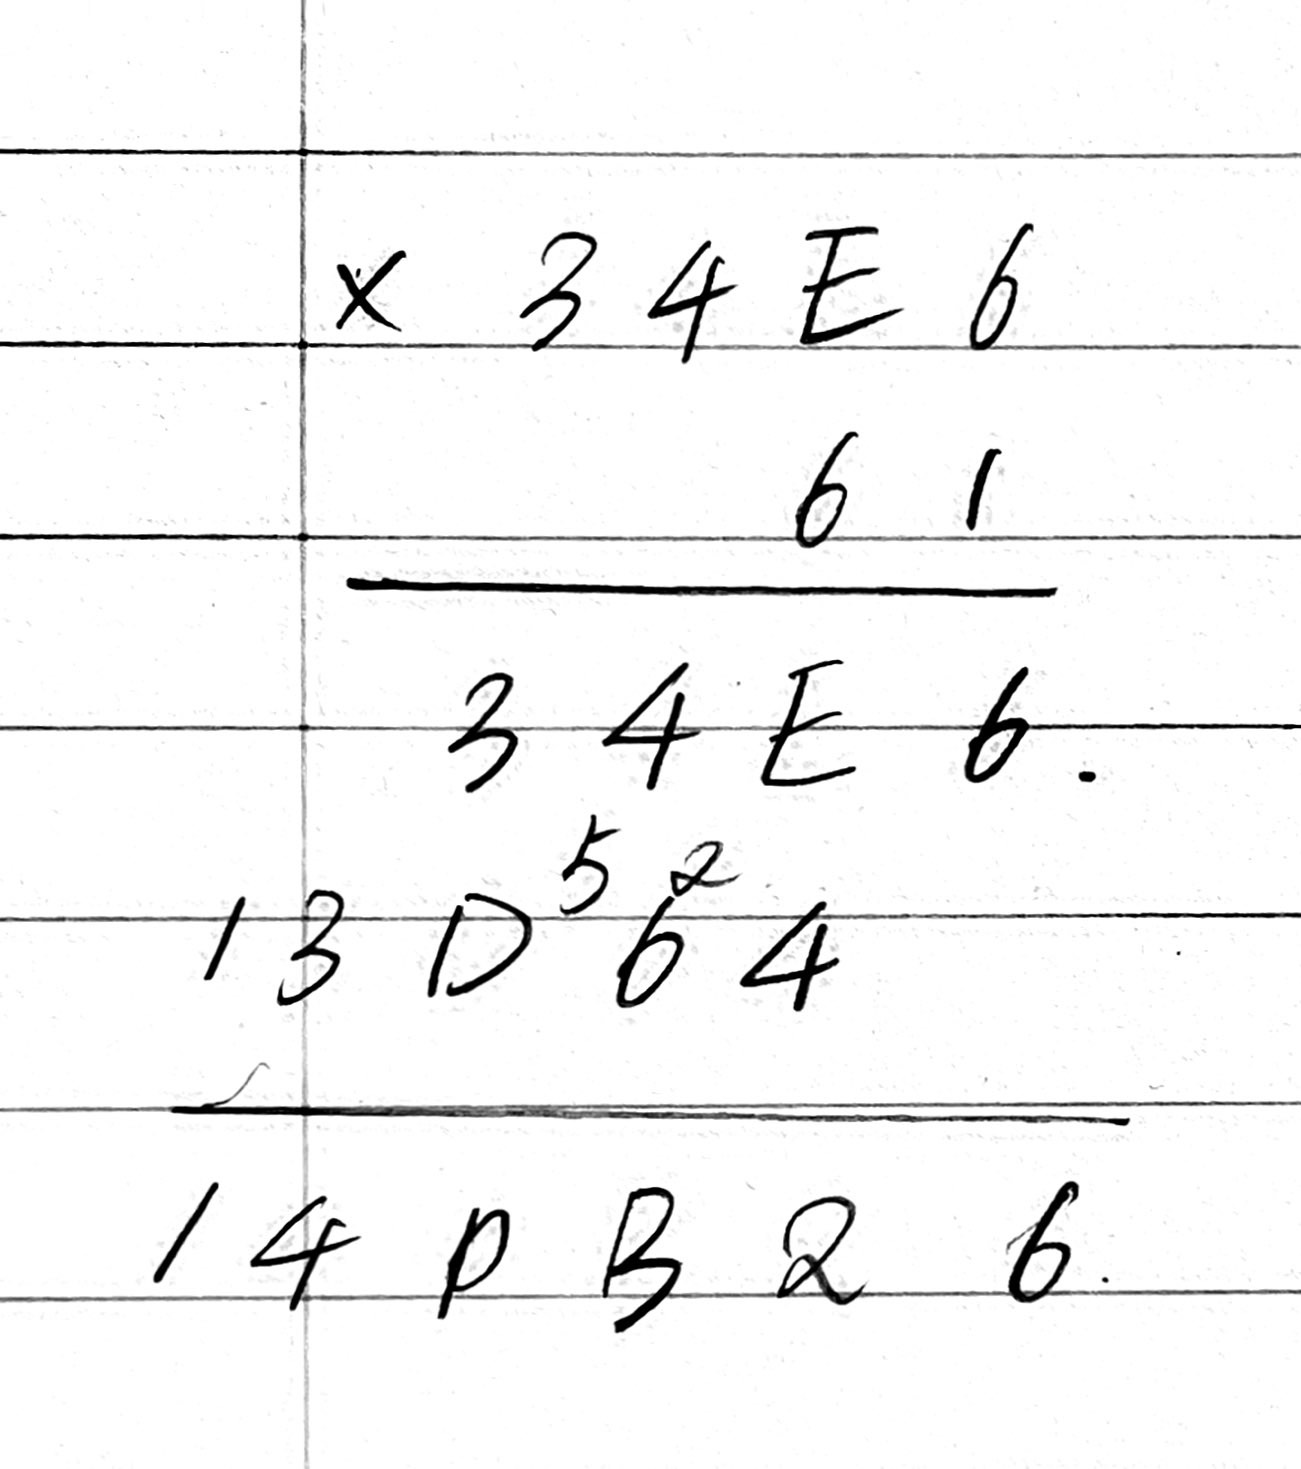
\includegraphics[width=0.3\textwidth]{hexmul.jpg} %插入图片,[]中设置图片大小,{}中是图片文件名
\caption{Hexdecimal Multiplication} 
\end{figure}

\section{}{B3: Matrices}
\subsection{Definition: Matrix}
Let $S$ be a set, and $m,n \; \in \mathbb{N}  $\\
An $m \times n \; matrix $ (over $S$) is a rectangular array of members of $S$,
the array having $m$ rows and $n$ columns. \\
The set of all $m \times n \; matrix $ matrices over $S$ is denoted by $M_{m \times n}(S)$\\
\section{D1:Graph Theory}
\subsection{Definition of Graphs}
A graph $G$ is an ordered pair $G = (V(G),E(G)) $ comprising:
\begin{itemize}
    \item a set of vertices $V(G)$
    \item a multiset of edges $E(G)$, with each edge being a size-2 multiset of vertices. 
\end{itemize} 
\subsection{Terminology}
\begin{itemize}
    \item An edge connects its \textbf{endpoints}.
    \item An edge with both endpoints the same is called a \textbf{loop}.
    \item Two edges may connect the same pair of endpoints, in which case they are said to be \textbf{parallel}.
    \item Two vertices are adjacent if they are connected by an edge; two edges are adjacent if they share an endpoint. 
    \item An edge is \textbf{incident on} its endpoints.
    \item A vertex with no incident edges is \textbf{isolated}.
    \item The \textbf{order} of a graph is the number of vertices. 
\end{itemize}
\subsection{Isomorphisms}
An \textbf{Isomorphism} between two graphs $G_1$ and $G_2$ is a bijection $f:V(G_1) \rightarrow V(G_2)$ such that $\{u,v\}$ appears in $E(G_1)$ exactly as many time as $\{f(u),f(v)\}$ appears in $E(G_2)$.
\subsection{Digraphs}
A directed graph is the same as a graph except that edges are ordered pairs of endpoints.
\subsubsection{Niche Overlap Graphs}
Application in ecology, each species is represented by a vertex. An undirected edge connects two vertices if and only if the species represented by these vertices compete for food.
\section{Types of Graphs}
\begin{itemize}
    \item A simple graph is a graph that has no loops and no parallel edges.
    \item A simple digraph is a digraph that has no loops and no parallel edges.\\
    \textbf{NOTE:} $(a,b)$ and $(b,a)$ is allowed. 
    \item A complete graph on $n$ vertices is a simple graph in which each pair of distinct vertices are adjacent. A complete graph on $n$ vertices is denoted by $K_n$.
    \begin{align}
        the \;number\; of\; edges = \frac{n(n-1)}{2} =\binom{n}{2} 
    \end{align}
    \item A bipartite graph is a simple graph whose vertices can be partitioned into two disjoint sets $A$ and $B$ such that every edge of the graph connects a vertex in $A$ to a vertex in $B$.
    \item A complete bipartite graph is a simple graph whose vertices may be partitioned into two sets $A$ and $B$ such that:\\
    $\forall a \in A$ and $\forall b \in B$, the edge $\{a,b\}$ belongs to the graph. 
    If $A$ has $m$ vertices and $B$ has $n$ vertices, the complete bipartite graph on $A$ and $B$ is denoted $K_{m,n}$ with $m \times n $ edges.
    
\end{itemize}
\subsection{Subgrah}
A subgrah,$S$, of a graph $G$, is a graph whose vertices are a subset of $V(G)$ and whose edges are a subset of $E(G)$. 
\begin{align}
    V(S) \subseteq V(G)\\
    E(S) \subseteq E(S)
\end{align}
\subsection{Degree}
The degree of a vertex is the number of edges incident on it(each loop counted twice). 
\subsection{The Handshake Theorem}
If $G$ is any graph, then the total degree of $G$ equals twice the number of edges of $G$.
\begin{align}
    \sum_{v \in V(G)} deg(v) = 2\left\lvert E(G) \right\rvert 
\end{align}
\textbf{NOTE:} It is impossible to have a graph has an even number of vertices of odd degree. 
\subsection{Closed Walks}
A walk $v_0,e_1,v_1,2_2,\dots,e_n,v_n$ is called a closed when $v_0 = v_n$. 
\subsection{Paths}
A path is a walk that does not repeat any edge.\\
A simple path is a path which does not repeat any vertex.
\subsection{Circuits}
A circuit is a closed path.\\
A simple circuit is a simple closed path.
\subsection{Connected Graphs}
A graph is connected if every pair of vertices can be connected by a walk.\\
A component of a graph is a maximal connected subgraph.
\subsection{Bridges and Cut vertices}
A bridge in a connected graph is an edge which erasure disconnects the graph. \\
A cut vertex in a connected graph is a vertex which one erasure disconnects the graph. 
\subsection{Euler Paths and Circuits}
Euler path: is a path passing through every edge.\\ 
Euler circuit: is a circuit passing through every edge.
\begin{thm}
    A connected graph has an Euler circuit if and only if each of its vertices has even degree. 
\end{thm}
\begin{corollary}
    A connected graph has an Euler path if and only if it has exactly two vertices of odd degree. 
\end{corollary}
\subsection{Fleury's Algorithm for finding Euler Circuits}
\begin{enumerate}
    \item Pick any vertex of $G$ as a starting point. 
    \item From that vertex choose any edge to traverse that does not cross a bridge of the current reduced graph, unless there is no choice.
\end{enumerate}
\subsection{Hamilton Paths and Circuits}
A Hamilton path for a graph is a simple path which passes through every vertex. 
A Hamilton circuit for a graph is a simple circuit which passes through every vertex. 
\subsection{Trees}
A tree is a connected graph with no circuits other that the trivial ones. 
\begin{thm}
    Let T be a graph with n vertices. The following statements are logically equivalent:
    \begin{enumerate}
        \item T is a tree.
        \item T has no simple circuits and n-1 edges.
        \item T is connected and has n-1 edges.
        \item T is connected and every edge is a bridge. 
        \item Any two vertices of T are connected by exactly one simple path. 
        \item T contains no non-trivial circuits, but the addition of any new edge creates a simple circuit. 
    \end{enumerate}
\end{thm}
\subsection{Spanning Tree}
A spanning tree for a graph $G$ is a subgraph of G which is a tree and contains all the vertices of $G$.  
\textbf{Method:}Initialize T to be the vertices of G but not edges, pick an edge and add to T if and only if it does not make a circuit in T. 
\section{D2:Weighted Graphs}
A weighted graph is a graph $G$ together with a weight function weight : $E(G) \rightarrow \mathbb{Q}_+ $. \\
Four type of problems in the weighted graphs:
\begin{enumerate}
    \item Minimal spanning tree:
    Find a spanning tree of least possible total weight.
    \item Find a Hamilton circuit of the least possible total weight.
    \item Find a path between two given vertices that has the least possible total weight.
    \item Maximum Flow 
\end{enumerate}
\subsection{Kruskal's algorithm for minimal spanning tree}
\textbf{Input:} Weighted connected graph $G$ with $n$ vertices.\\
\textbf{Output:} Minimal spanning tree $T$ for $G$. Total weight $W$ of this tree. \\
\textbf{Method:}Always select the minimum edge as long as there is no circuit formed when the new edge is added.\\ 
\textbf{NOTE}:This is an example of greedy algorithm and \textbf{always succeeds}. 

\subsection{The 'Nearest Neighbor' algorithm}
\textbf{Input:} Weighted \textbf{complete} graph $G$ with $n$ vertices.\\
\textbf{Output:} Hamilton circuit for $G$ as a list $L$ of vertices. Total weight $W$ of this circuit. \\
\textbf{Method:} Start with any vertex and choose a vertex $v$ such that weight of the edge as small as possible. Repeat this step until all the vertices are included.\\
\textbf{NOTE}:This is an greedy algorithm and does not \textbf{always succeed}. \\
\textbf{Example:}\\
\textit{Question: }There are 6 vertices and the graph is complete, how many possible Hamilton circuits exist?\\
With 6 vertices there are apparently 6! = 720 circuits, but allowing for different starting points and directions of travel, only 5!/2 = 60 are genuinely different.


\subsection{Dijkstra's Algorithm}
\textbf{Input:} 
\begin{itemize}
    \item Connected simple graph $G$. Vertices A,Z from $G$. 
    \item Distance function dist:$E(G) \rightarrow \mathbb{Q}^+$
\end{itemize}
\textbf{Output:}
\begin{itemize}
    \item Tree $T$ containing A and Z as vertices.
    \item $T$ is a subgrah of $G$. The unique path $A \rightarrow Z$ in $T$ has minimal total distance of all paths $A \rightarrow Z$ in $G$.
    \item Labelling $L:V(T) \rightarrow \mathbb{Q}_+; L(v)=min.dist(A \rightarrow v)$. 
\end{itemize}
\textbf{Method:} Start with the vertex A and find the adjacent vertices. If the vertex is unmarked, then mark them. If the vertex is marked select one with minimum value as the next current vertex.\\
\textbf{NOTE:} Vertex is locked in implies that we have found the path of minimum distance from the starting vertex A. The \textbf{fringe vertices} are those have been marked but not yet locked in. The spanning tree produced by Dijkstra's algorithm will not be minimal in general.

\subsection{Transport Networks}
\textbf{Flow:} The flow F is a function $E(D) \rightarrow \mathbb{Q}_+$, where $D$ is the digraph representing the network. However, each edge $e$ has a fixed capacity $C(e)$ whereas its flow $F(e)$ can vary, subject to constraints:
\begin{enumerate}
    \item Flow cannot exceed capacity. $[\forall e \in E(D) F(e) \le C(e).]$
    \item In each edge, flow direction = edge direction 
    \item Total flow into a node equals total flow out, except for nodes s’t (source, terminal).\\ 
    $[\forall v \in V(D) \backslash \{s,t\} \sum_{e\in v_{out}}F(e)=\sum_{e\in v_{in}}F(e)]$
\end{enumerate} 
\textbf{Input:} Transport network D with capacity function C.
\textbf{Output:} A Maximum flow function $F_{MAX}$ for the network.\\  
\textbf{Method:} \\
\textbf{NOTE:} Always go through the minimum terminal labelling first. 
\subsubsection{Applications of Transport Network in Matching Problems }
To the arrow diagram for the relation add an extra node s, the ‘super source’, and a link from s to each member of the domain of the relation. Then add another extra node t, the ‘super sink’ (super target), and a link to t from every member of the codomain of the relation. Now give all links a capacity of 1. A maximum flow now gives a maximal matching by picking all arrows from domain to codomain that have non-zero flow.
Remarks (not necessary for the answer to this question but relevant to the presentation of the solutions to the remaining questions):
\begin{enumerate}
    \item Since all links have capacity 1, it is not necessary to display capacities.
    \item Since a link with capacity 1 is either fully used or not used at all, rather than show
    spare capacity and flow we can show used/unused.
    \item Similarly, there is no need to show potential flow values on vertex labels.
    \item My convention will be show used links by heavy lines.
    \item When a link AZ from domain to codomain is used, the links sA and Zt must also be used, so there is no logical need to mark them. However, marking them helps to avoid making mistakes in annotating vertices, so I will still mark them, but less thickly.
\end{enumerate}
\textbf{NOTE:}
Start with codomain in alphabetical order. 

\section{D3: Random Walks on Graphs}
\subsection{Definition:Random Walks}
Let G be a digraph with n vertices $V = V(G) = \{1,\dots,n\}$ and directed edge set $E = E(G)$. 

A square matrix with non-negative entries such that the enties in each row sum to 1 is called a stochastic matrix. 

Basis vectors : elementary vectors. For any given n, let $B_n$ denote the set of basis vectors $\{e_1,\dots,e_n\}$ where $e_i$ is the $n \times 1 $ vector with 1 as the i-th entry and all other entries zero. 

For $X_0=e_i \in B_n$ the sequence $(X_k)_{k \in \mathbb{N^*}} $
specified by $G$ and $T$ is called the random walk on G starting at vertex $i$ with transition matrix $T$. 

Then $X_k = (T')^k e_i = (q_j)_{1 \le j \le n}$ say gives, for $1 \le j \le n$, the probability $q_j$ of being at the vertex $j$ after $k$ steps, starting form vertex $i$. 
\section{Method of Calculating Steady States}
\begin{enumerate}
    \item Write out the transition matrix $T$. 
    \item Transpose the matrix $T$ to $T'$.
    \item Subtract the identity matrix from the transposed matrix $T'$. 
    \item Add columns with all entries 0 after the last column of matrix. 
    \item \textbf{Replace} the last tow with all 1's
    \item Apply the row operations to reduce the matrix to row reduced echelon form and the last column is the steady states. 
\end{enumerate}
\subsection{HYPOTHESES OF THE MODEL}
\begin{enumerate}
    \item Each link to $W$ is saying that $W$ is a bit awesome.
    \item A link to $W$ from an awesome page is saying more than a link to $W$ from a less awesome page.  
\end{enumerate}
\subsection{The Structure of an Internet}
Represent an internet as a digraph called \textbf{webgraph}. The vertices represent of the web, and there is a directed edge from verttex $X$ to vertex $Y$ if and only if there is a hyperlink from the page corresponding to $X$ to the page corresponding to $Y$. 
\subsection{Introduce Damping Factor}
\begin{enumerate}
    \item With the probability $\alpha$, the RS will type in the URL of a randomly chosen page(unforced teleporting).
    \item With probability $(1-\alpha)$ the RS will proceed as follows: if there is at least one hyperlink on the current page, the RS will choose at random one of the these hyperlinks and click on it; if there is no hypoerlink on the current page, then the RS will choose a new page at random(forced teleporting).
\end{enumerate}
\subsection{PageRank}
Let $P = (p_1,p_2,\dots,p_n)$ be the steady state vector for the random walk on $W$ using the transition matrix $M$. For each $i \in \{1,\dots,p_i\}$, $p_i$ is the PageRank of page $i$. 
\subsection{Modified Probability for Transition from vertex i to j}
\begin{align}
        m_{ij} = \alpha/n + (1-\alpha)t_{ij}\\
        M = (m_{ij})_{1 \le i,j \le n} = (\alpha/n+(1-\alpha)t_{ij})_{1 \le i,j \le n}\\
        = (\alpha/n)U +(1-\alpha)T
\end{align}
\subsection{Calculating PR}
\begin{align}
    (I-(1-\alpha)T')PR = (\alpha/n)1
\end{align}
\subsection{iterative Approximation Method}
\begin{align}
    P_0 = (1/n)1; P_k =\alpha P_0+(1-\alpha)T'P_{k-1}, k \ge1.
\end{align}

\section{C3:Markov Process}
It is closely related with the above topic. 
\subsection{Steady State vector}
\begin{align}
    T'v=v
\end{align}

\begin{thm}
Let $T = (T_{ij})_{1 \le i,j \le k}$ be the transition matrix for a $k$ state Markov process with state vectors $x_n,n \in \mathbb{N} $. Then $\forall n \le 1$:
\begin{enumerate}
    \item $x_n = T'x_{n-1}$
    \item $(T^n)_{ij} is  \;the \;n-step \;i-to-j \; transition\; probability.$
    \item $x_n = (T')^n x_0$
\end{enumerate}
\end{thm}

\end{spacing}
\end{document}

